\documentclass{letter}

\usepackage{csquotes}
\usepackage[margin=1in]{geometry}
\usepackage{tikz}
\usepackage{amsmath}
\usepackage{enumitem}

\newcommand{\heading}[1]{{\large \textsc{#1}}}

\begin{document}

\heading{COMP 282 - Quiz 1 (Spring, 2019)}
\kern 2cm
\heading{Name:}

{\bf Question 1} \kern 1cm Arrange the following classes of functions (in Big-O
notation) in {\em increasing} order:

\begin{enumerate}[label=(\alph*)]
\item $O(n)$
\item $O(2^n)$
\item $O(n\lg n)$
\item $O(n^2)$
\item $O(1)$
\end{enumerate}

{\bf Question 2} \kern 1cm Give a formal definition for the following graph:

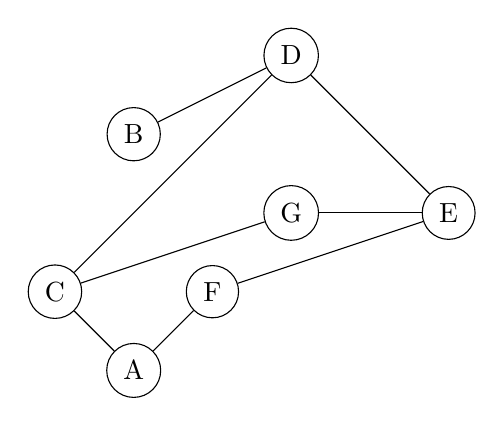
\begin{tikzpicture}
\node[shape=circle,draw=black] (A) at (1,1) {A};
\node[shape=circle,draw=black] (B) at (1,4) {B};
\node[shape=circle,draw=black] (C) at (0,2) {C};
\node[shape=circle,draw=black] (D) at (3,5) {D};
\node[shape=circle,draw=black] (E) at (5,3) {E};
\node[shape=circle,draw=black] (F) at (2,2) {F};
\node[shape=circle,draw=black] (G) at (3,3) {G};

\path (A) edge (C);
\path (A) edge (F);
\path (C) edge (D);
\path (C) edge (G);
\path (D) edge (B);
\path (D) edge (E);
\path (E) edge (F);
\path (E) edge (G);
\end{tikzpicture}

{\bf Question 3} \kern 1cm Fill in the rest of the table:

\begin {tabular}{ l | c | c | c | c }
    Data Structure & Insert & Delete & Search & Sort \\
    \hline
    Linked List & (a) & $O(n)$ & (b) & $O(n\lg n)$ \\
    Array & (c) & (d) & (e) & $O(n\lg n)$ \\
\end{tabular}

\begin{enumerate}[label=(\alph*)]
\item
\item
\item
\item
\item
\end{enumerate}

{\bf Question 4} \kern 1cm Draw the graph, given by the following formal definition:

$G = (V, A)$

$V = \{ a, b, c, d, e \}$ 

$A = \{ (a,c), (b,c), (c,a), (c,d), (d,b), (d,e), (e,a), (b,a) \}$

\end{document}
